\documentclass[a4paper,hidelinks,14pt]{extarticle}

\usepackage[utf8]{inputenc}
\usepackage[T2A]{fontenc}
\usepackage[english, russian]{babel}
\usepackage{lipsum}
\usepackage{amsmath}
\usepackage{amssymb}
\usepackage{amsfonts}
\usepackage{mathtools}
\usepackage{datetime}
\usepackage[pdftex]{graphicx}
\usepackage{indentfirst}
\usepackage{asymptote}
\usepackage{systeme}
\usepackage[dvipsnames]{xcolor}
\usepackage{lastpage}
\usepackage{fancybox,fancyhdr}
\usepackage{hyperref}
\usepackage[font={small,it}]{caption}

\usepackage{minted, xcolor}
\usemintedstyle{monokai}
\definecolor{bg}{HTML}{282828}
\setminted{bgcolor=bg}
\setminted{fontsize=\scriptsize}
\setminted{}

\fancyhead[R]{\textit{Отчет о практике}}
\fancyfoot[L]{}
\fancyfoot[C]{Страница \thepage\space из \pageref{LastPage}}
\fancyfoot[R]{}
\pagestyle{fancy}
\setlength{\headheight}{17.0pt}


\fancypagestyle{nofooter}{
	\fancyhead[R]{\textit{Отчет о практике}}
	\fancyfoot[L]{}
	\fancyfoot[C]{}
	\fancyfoot[R]{}
}

\newcommand{\anonsection}[1]{\section*{#1}\addcontentsline{toc}{section}{#1}}


\begin{document}
	\begin{titlepage}
		\setlength{\parindent}{0ex}
		
		\begin{center}
			\textsc{
				\vspace{1ex}
				Научно исследовательский университет ИТМО \\
				\vspace{0.5ex}
				Факультет систем управления и робототехники \\
				\vspace{0.5ex}
			}
		\end{center}
		
		\vspace{25mm}
		
		\begin{center}
			\large\textbf{Отчет} \\
			о производственной  \\
			научно-исследовательской практике \\
			\vspace{5mm}
			Разработка системы распознавания биометрии лица для робота-ассистента
		\end{center}
		
		\vspace{40mm}
		
		\begin{minipage}{.49\linewidth}
			Выполнил студент группы R3280
			
			Руководитель практики
		\end{minipage}
		\hfill
		\begin{minipage}{.5\linewidth}
			\begin{flushright}
				Мовчан Игорь Евгеньевич
				\\
				 Афанасьев Максим Яковлевич
			\end{flushright}
		\end{minipage}
		\vfill
		\begin{center}
			Санкт-Петербург
			\\
			2024
		\end{center}
		
	\newpage
	\thispagestyle{nofooter}
	\tableofcontents
	
	\end{titlepage}
	
	
	\anonsection{Введение}
	Трудно не согласиться с тем, что в последнее время машинное и глубокое обучение набирают всё большие и большие обороты, становясь важной частью человеческого мира за счёт автоматизации многих рутинных задач, на которые раньше уходило множество ресурсов (в том числе и человеческих). Чего только стоит один chatgpt, который за несколько секунд поможет ответить пользователю на большинство его вопросов, начиная с того, чего бы тебе такого вкусного поесть на ужин, и заканчивая кодингом и средней математикой (а это ещё пятая версия не вышла). Есть и множество других средств, которые умеют и картины писать (midjourney, stable diffusion), и песни сочинять (suno ai), и картины оживлять (lumalabs, runway ai)... Впрочем, всё это очередные восхваления, истинная суть которых на самом деле в том, что перед каждым из нас открываются всё более новые и интересные возможности буквально каждый сезон, и в во всём этом новом отдельное, эталонное место выделено машинному обучению.
	
	Итак, одна из интереснейших проблем, которую уже решило глубокое обучение, - распознавание биометрии лица человека. И в этом проекте мы как раз-таки посмотрим на неё изнутри, разработав систему такого распознавания для робота-ассистента Патрика, обладающего микрокомпьютером Khadas VIM3 в качестве <<головного отделения>>, и Ubuntu 20.04. 
	
	Суть системы заключается в <<чтении лица>> с потока камеры и последующем обновлении внутренней базы данных (то есть добавлении биометрии лица человека, если у нас ещё нет никакой информации о нём, и <<записи>> его посещения, если мы его уже <<знаем>>). Такая программа может использоваться, например, при создании системы входа сотрудников какой-либо организации или, как в нашем случае, при создании робота ассистента, которому важно знать, с кем он вступает (или уже вступал) в диалог.
	
	Разобравшись, зачем мы вообще всем этим занимаемся, приступим к самой практике!
	
	\newpage
	\section{Собираем информацию}
	Написание программы будет происходить на python, что в значительной степени облегчит нам работу с кодом, ведь на языке уже реализовано множество библиотек (в том числе с обученными сетями для всех этапов распознавания лица), реализующих чуть ли не всё, что только захочет сделать человек. Для наших же целей мы воспользуемся библиотекой face\_recognition, совмещающей в двух своей функцих compare\_faces, face\_encodings все этапы сравнения двух лиц. Но прежде давайте чуть поговорим об этих этапах, чтобы понимать, что за нашими используемыми функциями на самом деле стоит вполне ясный алгоритм действий:
	\begin{enumerate}
		\item Поиск лиц (рис. \ref{1}). Пожалуй, есть два алгоритма решения проблемы - HOG и CNN. Первый использует градиенты (то есть происходит сравнение по яркости каждого отдельного пикселя и его соседей) и на полученном градиентном изображении находит похожий на выявленный при обучении паттерн лица человека. Второй, соответственно, сверточные нейронные сети. HOG - более производительный, CNN - более точный.
		\begin{figure}[h]
			\centering
			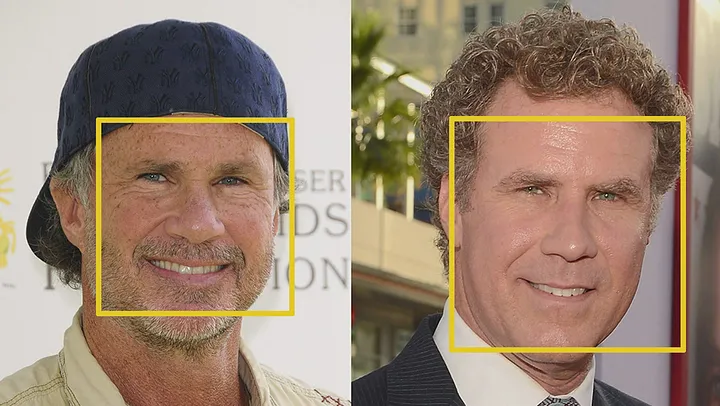
\includegraphics[scale=0.475]{im1.png}
			\caption{Поиск лиц на изображении}
			\label{1}
		\end{figure}
		\item <<Центрирование>> лица (рис. 2). Полученное лицо центрируется за счёт выделения специальных точек (границ) на лице человека с помощью заранее обученной сети и последующего преобразования изображения известными математическими методами преобразования пространства.
		\begin{figure}[h]
			\centering
			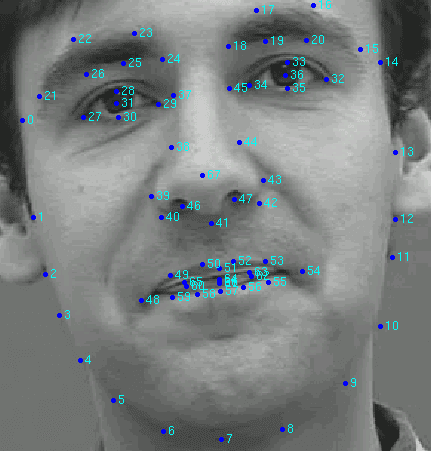
\includegraphics[scale=0.3]{im2.png}
			\caption{Поиск опорных точек на лице}
			\label{2}
		\end{figure}
		\item Снятие замеров с полученного лица. То, какие данные нужно измерения необходимо производить с лицом, чтобы получать наибольшую точность в распознавании, опять ложиться на нейронные сети.
		\begin{figure}[h]
			\centering
			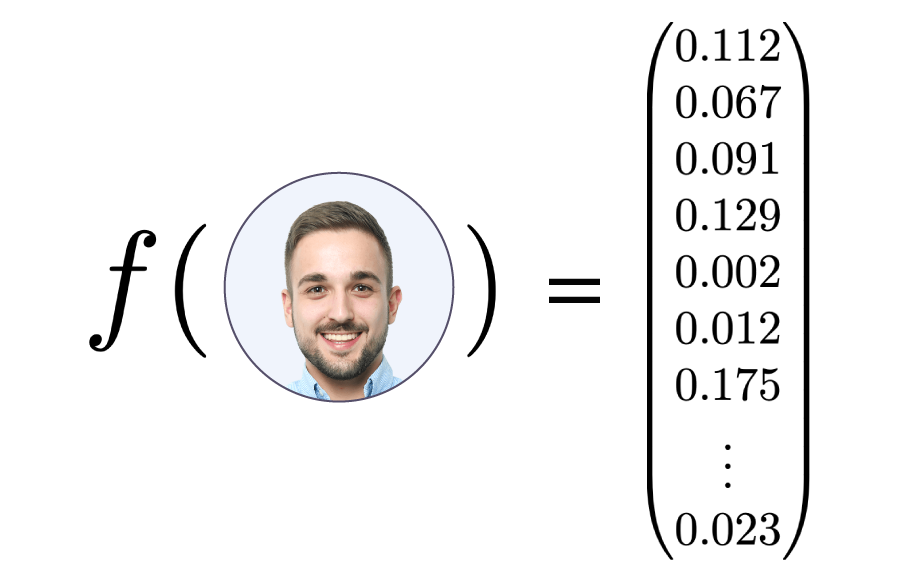
\includegraphics[scale=0.3]{im3.png}
			\caption{Поиск опорных точек на лице}
			\label{3}
		\end{figure}
		\item Вычисление <<дистанции>> между взятыми на предыдущем шаге данными и уже известными лицами, которые уже находятся в системе (ближайшая точка - данные, с которыми мы наиболее сходимся). Делается это с помощью обычных классификаторов (подойдёт даже k-means).
	\end{enumerate}
	
	С помощью вышеописанных шагов можно выяснить, что за человек находиться на изображении, если у нас уже есть набор известных нам людей. Изучив, как именно работает распознавание, переместимся непосредственно к реализации нашей системы!
	
	\section{Делаем!}
	\subsection{Базовая реализация}
	Итак, базовая реализация заключается в покадровом сравнии изображения с камеры и уже известных нам лиц (пусть они будут располагаться, например, в директории images нашего исходного проекта). Так как всё будет происходить life-time, то важно, чтобы сравнение происходило за максимально быстрый период времени, а значит, в реализации функции compare\_faces должен быть задействован метод HOG выделения лиц, дающий большую производительность (благо он уже установлен по умолчанию):
	\begin{minted}{python}
def compare_faces(faces_list: list[np.ndarray], face: np.ndarray, 
				  tolerance: float = 0.6) -> (bool, int):
	face_distances = face_recognition.face_distance(faces_list, face)
	match_index = np.argmin(face_distances) if face_distances.size else -1
	return (match_index >= 0 and face_distances[match_index] <= tolerance), match_index
	\end{minted}
	
	В этом коде вычисляется та самая <<дистанция>> между замерами лиц и делается предположение, схожи ли эти лица (если да, то возвращается индекс наиболее похожего лица). Переменная как tolerance показывает, какое расстояние между объектами считать достаточно близким для совпадений лиц.
	
	Функция compare\_faces является \textit{ключевой} при работе программы:
	
	\begin{minted}{python}
def main(camera_channel: int, exit_key: int,
         text_color: tuple = (0, 255, 0), frame_color: tuple = (255, 0, 0)) -> None:
	camera = cv2.VideoCapture(camera_channel)

	known_faces = []
	known_faces_name = []
	directory_path = "images/"
	files = [f for f in os.listdir(directory_path)
			 if re.match(r'.*\.(jpg|jpeg|png)', f, flags=re.I)]
	# извлечение из подготовленных изображений измерений лиц
	for f in files:
		filepath = os.path.join(directory_path, f)
		img = cv2.imread(filepath)
		img_rgb = cv2.cvtColor(img, cv2.COLOR_BGR2RGB)
		enc = face_recognition.face_encodings(img_rgb)
		if enc:
			measurements = enc[0] # взятие только одного лица
			known_faces.append(measurements)
			name = "".join(f.split(".")[:-1])
		known_faces_name.append(name)

	while True:
		# чтение потока с камеры
		result, frame = camera.read()

		# отзеркаливание (для удобства)
		flipped_frame = cv2.flip(frame, 1)
		# конвертирование цвета изображения в rgb (opencv работает с brg)
		rgb_flipped_frame = cv2.cvtColor(flipped_frame, cv2.COLOR_BGR2RGB)
		# выделение лиц с полученного кадра
		face_locations = face_recognition.face_locations(rgb_flipped_frame)
		face_encodings = face_recognition.face_encodings(rgb_flipped_frame, face_locations)
	
		# последовательная обработка выделенных лиц
		face_names = []
		for face_enc in face_encodings:
			res, index = compare_faces(known_faces, face_enc)
			# присваивание имени
			name = "Unknown"
			if res:
				name = known_faces_name[index]
			face_names.append(name)

		for loc, name in zip(face_locations, face_names):
			top, right, bottom, left = list(loc)
			# отрисовка "квадратов" вокруг лиц
			cv2.rectangle(flipped_frame, (left, top), (right, bottom), text_color, 3)
			font = cv2.FONT_HERSHEY_TRIPLEX
			cv2.putText(flipped_frame, name, (left + 6, bottom - 6),
					    font, 1.0, frame_color)

		cv2.imshow("Face Recognition", flipped_frame)

		# выход на esc
		key = cv2.waitKey(1)
		if key == exit_key:
			break	
		
		camera.release()
		cv2.destroyAllWindows()
		
	\end{minted}
	
	В результате выполнения программа прогоняет каждый кадр через выделение лиц на нём, снятие измерений и сопоставление с уже известными лицами, а после добавляет рамку вокруг лица на этот кадр. На выходе получаем работоспособную программу с одним нюансом (!) - она работает достаточно медленно. Каждый кадр обрабатывается более чем четверть секунды, и это приводит к тому, что на выходе мы получаем дёрганый видеопоток (а хотелось бы получить более плавный; видео с примером работы (как и сама программа) загружено на \href{https://github.com/ventusjke/attendance_system/tree/main/practice_videos/basic.mkv}{github}).
	
	\subsection{Оптимизация}
	Добиться большей производительности поможет \textit{сжатие} полученных изображений с камеры и взятие, например, каждого второго кадра из потока:
	
	\begin{minted}{python}
# добавляем счётчик на кадры, если достигаем лимита - обрабатываем и обнуляем
frame_counter = 0
while True:
	result, frame = camera.read()
	flipped_frame = cv2.flip(frame, 1)
	frame_counter += 1

	if frame_counter >= frame_counter_limit:
		# сжимаем кадр в 1/compression_ration раз
		small_flipped_frame = cv2.resize(flipped_frame, (0, 0), fx=1/compression_ratio,
									fy=1/compression_ratio)
		rgb_flipped_frame = cv2.cvtColor(small_flipped_frame, cv2.COLOR_BGR2RGB)
		face_locations = face_recognition.face_locations(rgb_flipped_frame)
		face_encodings = face_recognition.face_encodings(rgb_flipped_frame, face_locations)

		face_names = []
		for face_enc in face_encodings:
			res, index = compare_faces(known_faces, face_enc)
			name = "Unknown"
			if res:
				name = known_faces_name[index]
			face_names.append(name)
		frame_counter = 0 # сброс счётчика в 0

	if face_locations and face_names:
		for loc, name in zip(face_locations, face_names):
			# заново растягиваем, чтобы получить рамку именно вокруг лица
			upd_loc = map(lambda x: x * compression_ratio, list(loc))
			top, right, bottom, left = upd_loc
			cv2.rectangle(flipped_frame, (left, top), (right, bottom), text_color, 3)
			font = cv2.FONT_HERSHEY_TRIPLEX
			cv2.putText(flipped_frame, name, (left + 6, bottom - 6),
				    font, 1.0, frame_color)
	\end{minted}
	
	Тесты показывают, что каждый кадр в базовой реализации обрабатывается где-то за $0.35$ секунд, тогда как в оптимизированной программе (\href{https://github.com/ventusjke/attendance_system/blob/main/practice_videos/optimized.mkv}{видео}) - за 0.25 (при сжатии в 3 раза), если же к этому прибавить то, что мы обрабатываем, например, каждый второй кадр, то мы получаем прирост в производительности почти в $2.5$ раза, если считать время на обработку двух последовательных кадров.
	
	\subsection{База данных}
	Наша система должна хранить данные о пользователях во внутренней базе данных. Казалось бы, идеальным кандидатом на такую роль для нашего робота-ассистента с его микрокомпьютером стала бы sqlite, которая имеет ряд преимуществ в виде легковесности, чуть более быстрой работе с одним пользователем и в целом чуть меньшим потреблением по сравнению с другими базами данных. Однако тут возникает вопрос: как нам хранить данные об уже известных людях. Конечно, можно хранить всё в каком-нибудь внутреннем файле, но, кажется, это не очень гигиенично, а при большом количестве пользователей мы и вовсе будем терпеть крах в виде медленной работы (которую, правда, можно ускорить за счёт многопоточности).
	
	Итак, было решено использовать вместо sqlite postgresql и организовать полное хранение, включая записи о посещениях и измерения лиц для каждого отдельного человека, в соответствующих таблицах.
	
	Для управления базой данных был создан отдельный модуль с единственным классом Database внутри. По сути мы лишь переместили управление нашими данными в выделенную сущность:
	\begin{minted}{python}
class Database:
	def __init__(self, dbname: str = "users", user: str = "postgres", password: str = "",
				 host: str = "127.0.0.1", port: str = "5432"):
		# устанавливаем соединение с базой данных (users по умолчанию)
		self.connection = psycopg2.connect(
			host=host,
			dbname=dbname,
			user=user,
			password=password,
			port=port
		)
		# берём курсор для запуска команд
		self.cursor = self.connection.cursor()

	def create_users_table(self) -> None:
		# создание таблицы с пользователями, в которой хранятся id, 
		# дата последнего распознавания и их общее количество, а также биометрия
		self.cursor.execute("""
		CREATE TABLE IF NOT EXISTS users_info (
			id SERIAL PRIMARY KEY,
			total_attendance INTEGER,
			last_attendance TIMESTAMP WITH TIME ZONE,
			img_enc NUMERIC[]
		);
		""")
		self.connection.commit()

	def add_images_to_database(self, directory_path: str) -> None:
		# добавление изображений в базу данных с реализацией, которая была в базовой версии
		files = [os.path.join(directory_path, file) for file in os.listdir(directory_path)
				 if re.match(r'.*\.(jpg|jpeg|png)', file, flags=re.I)]
		for file in files:
			img = cv2.imread(file)
			img_rgb = cv2.cvtColor(img, cv2.COLOR_BGR2RGB)
			enc = face_recognition.face_encodings(img_rgb)
			if enc:
				measurements = enc[0]
			self.cursor.execute("""
			INSERT INTO users_info (total_attendance, last_attendance, img_enc)
			VALUES (%s, %s, %s);
			""", (0, datetime.now(), measurements.tolist()))
		self.connection.commit()

	def make_sql_request(self, sql_request: str, data: tuple = None) -> None:
		self.cursor.execute(sql_request, data)
		self.connection.commit()

	def fetchall(self) -> list: # для извлечения данных из запроса
		return self.cursor.fetchall()

	def close(self) -> None:
		if self.connection:
			self.connection.close()
		if self.cursor:
			self.cursor.close()

	\end{minted}
	
	Также в основной функции нам не нужно каждый раз отдельно считывать изображения, ведь они уже хранятся в нашей базе данных (а ещё у нас появилась возможность вручную обновлять данные в программе и даже добавлять новых пользователей, запуская одновременно код на разных видеоканалах, что может нам понадобиться при дальнейшей расширении функционала). Вот все изменения, которые произошли в коде функции main:
	
	\begin{minted}{python}
database = Database(**database_settings)
database.create_users_table()
database.add_images_to_database("images/")
camera = cv2.VideoCapture(camera_channel)
...
if frame_counter >= frame_counter_limit:
	database.make_sql_request("SELECT id, img_enc FROM users_info")
	faces = dict(database.fetchall()) # словарь имя: биометрия
	...
	\end{minted}
	 
	
	\subsection{Запоминание и записи о появлении}
	Пожалуй, самым важным свойством нашей программе является её динамичность (то есть возможность прямо во время работы запомнить пользователя в базу данных и распознавать его). Стоит отметить, что у анализатора лиц случаются <<промашки>>, поэтому, пожалуй, самым лучшим способом будет запоминать (да и отмечать) лицо спустя какое-то время (или спустя $N$-ое количество обработанных кадров). Что ж, так и поступим:
	
	\begin{minted}{python}
database.create_users_table()
database.create_records_table()
...
# счётчик-словарь (id: count) на известные лица
known_faces_counter = {}
# cчётчик-список с элементами tuple (число вхождений, биометрия) на неизвестные лица
unknown_faces_counter = []
face_locations = []
face_names = []
while True:
	res, frame = camera.read()
	flipped_frame = cv2.flip(frame, 1)
	frame_counter += 1

	if frame_counter >= frame_counter_limit:
		...
		face_names = []
		temp_known_counter = {}
		temp_unknown_counter = []
		for face_enc in face_encodings:
			res, index = compare_faces(known_faces, face_enc)
			name = "Unknown"
			if res:
				name = known_faces_name[index]
				# если нашли знакомое лицо - прибавляем счётчик,
				# если нет - добавляем в словарь с 0 вхождений
				temp_known_counter[name] = known_faces_counter.get(name, 0) + 1
			else:
				unknown_faces = [face for count, face in unknown_faces_counter]
				res, index = compare_faces(unknown_faces, face_enc)
				# сравнение лиц, находящихся на этапе запоминания с обрабатываемым
				count = unknown_faces_counter[index][0] if res else 0
				# если есть схожести - увеличение счётчика,
				# если нет - добавление нового элемента
				temp_unknown_counter.append((count + 1, face_enc))
			face_names.append(str(name))
		# временные переменные используются для удаления старых лиц, 
		# которые мы не нашли на обрабатываемом кадре
		known_faces_counter = temp_known_counter
		# процесс регистрации распознавания, добавление записи о вхождении
		# в таблицу records (id INTEGER, attendance_time TIMESTAMP)
		# о посещениях пользователей
		names = []
		for name in known_faces_counter:
			# remember_counter_limit задаёт то, сколько обработанных подряд
			# кадров нам понадобится для регистрации вхождения
			if known_faces_counter[name] >= remember_counter_limit:
				names.append(name)
				database.make_sql_request("""
					UPDATE users_info
					SET total_attendance = total_attendance + 1,
					last_attendance = %s WHERE id = %s;""",
					(datetime.now(), name))
				# добавление записи в records
				database.make_sql_request("""
					INSERT INTO records (id, attendance_time)
					VALUES (%s, %s);""", (name, datetime.now()))
				print(f"{name} attendance was approved!")
		# удаление зарегистрированных
		for name in names:
			known_faces_counter.pop(name)
			
		unknown_faces_counter = temp_unknown_counter
		# процесс запоминания пользователя
		indexes = []
		for i in range(len(unknown_faces_counter)):
			count, unknown_face = unknown_faces_counter[i]
			# recognize_counter_limit задаёт то, сколько обработанных подряд
			# кадров нам понадобится для запоминания пользователя
			if count >= recognize_counter_limit:
				indexes.append(i)
				database.make_sql_request("""
					INSERT INTO users_info
					(total_attendance, last_attendance, img_enc)
					VALUES (%s, %s, %s);""",
					(1, datetime.now(), unknown_face.tolist()))
				database.make_sql_request("SELECT MAX(id) FROM users_info;")
				# добавление вхождения в records
				name = database.fetchall()[0]
				database.make_sql_request("""
					INSERT INTO records (id, attendance_time)
					VALUES (%s, %s);""", (name, datetime.now()))
				print(f"new face added to db!")
		# удаление запомненных
		for index in indexes:
			unknown_faces_counter.pop(index)
	\end{minted}
	\newpage
	В класс управления базой данных также был добавлен метод для создания таблицы записей records:
	\begin{minted}{python}
def create_records_table(self) -> None:
	self.cursor.execute("""
		CREATE TABLE IF NOT EXISTS records (
			id INTEGER,
			attendance_time TIMESTAMP WITH TIME ZONE
		);
		""")
	self.connection.commit()
	\end{minted}
	
	Видео с результатом запоминания можно посмотреть по \href{https://github.com/ventusjke/attendance_system/blob/main/practice_videos/memorization.mkv}{ссылке} (сжатие и пропуск кадров были выставлены на 3) на \href{https://github.com/ventusjke/attendance_system}{github программы}.
	
	На этом, пожалуй, всё!
	
	
	\newpage
	\anonsection{Выводы}
	В результате работы над практическим заданием была получена жизнеспособная система (со своей базой данных) распознавания биометрии лица человека, являющаяся довольно-таки быстрой и точной, извлечён гигантский опыт в области ML, получено множество полезных практических и не только навыков, изучено, как работает распознавание лиц людей и обработка видеопотока. Могу с уверенностью сказать, что приобретённые в процессе выполнения работы знания не пропадут зря!
	\newpage
	\anonsection{Список используемых источников}
	\begin{enumerate}
		\item \href{https://medium.com/@ageitgey/machine-learning-is-fun-part-4-modern-face-recognition-with-deep-learning-c3cffc121d78}{Machine Learning is Fun! Part 4 by Adam Geitgey}
		\item \href{https://www.geeksforgeeks.org/convolutional-neural-network-cnn-in-machine-learning/}{Convolutional Neural Network (CNN) in Machine Learning}
		\item \href{https://github.com/ageitgey/face_recognition}{github of face\_recognition library}
		
	\end{enumerate}
	
	
\end{document}